\documentclass[10pt,a4paper]{article}
\usepackage[margin=2cm]{geometry}
\usepackage[T1]{fontenc}
\usepackage{lmodern}
\usepackage{booktabs}
\usepackage{graphicx}
\usepackage{amsmath}
\usepackage[font=small,labelfont=bf]{caption}
\usepackage{xcolor}
\usepackage{placeins}
\usepackage{tocloft}
\usepackage{rotating}
\setlength{\cftsecnumwidth}{2.6em}
\usepackage[colorlinks=true,linkcolor=blue!50!black,urlcolor=blue!50!black]{hyperref}
\renewcommand{\thetable}{S\arabic{table}}
\renewcommand{\thefigure}{S\arabic{figure}}
\renewcommand{\thesection}{S\arabic{section}}
\setlength{\parindent}{0pt}\setlength{\parskip}{4pt}
\newsavebox{\tabbox}
\newcommand{\fit}[1]{\sbox{\tabbox}{#1}\ifdim\wd\tabbox>\linewidth\resizebox{\linewidth}{!}{\usebox{\tabbox}}\else\usebox{\tabbox}\fi}
\setcounter{secnumdepth}{2}
\title{Supplementary Material for: Unseen-Attack Detection in the Internet of Medical Things: A Leave-One-Attack-Out Evaluation of Sequence Models, Energy Scores and Feature-Space Profiles}
\author{Sudhir Kumar Sharma\textsuperscript{1} and Sneha Vasishth\textsuperscript{2}\\[4pt]
{\small \textsuperscript{1}Sharda School of Computing Science and Engineering, Sharda University, Greater Noida 201310, India}\\
{\small \textsuperscript{2}LeewayHertz, Department of Data Science, Sector 47, Gurugram, Haryana, 122001, India}}
\date{}
\begin{document}
\maketitle
\begin{center}\itshape Supplementary material for peer review. All analyses here are exploratory or descriptive unless stated; none changes any H1--H5 verdict of the manuscript.\end{center}
\tableofcontents
\clearpage
\section{Overview}\label{sec:n1}
This document gives the details behind the analyses summarized in the manuscript. Every table is generated by script from the stored result files. Section references in the text refer to the manuscript, for example Section~V-F (ESA1).
Unless a caption says otherwise, the analyses are exploratory or descriptive and do not change any verdict of H1--H5. Class and architecture names are those of the manuscript: ARP spoofing, Recon-VulScan, malformed MQTT traffic, TCP/IP DoS-UDP and MQTT-DDoS publish flooding; TRACE-MoE, Transformer and BiLSTM-DNN. Results are means over the five seeds 42 to 46 unless stated.
\begin{center}\small\begin{tabular}{@{}lll@{}}\toprule Section & Content & Manuscript section\\ \midrule
\ref{sec:n2} & Training configuration, test-window counts & Experimental Setup\\
\ref{sec:n3} & Inference benchmark & Inference Overhead\\
\ref{sec:n4} & Safety-view decomposition & H1 results\\
\ref{sec:n5} & Threshold calibration, Benign alerts, event-level rule & Section~V-F (ESA1)\\
\ref{sec:n6} & Agreement of energy and MSP rankings & Section~V-G (ESA2)\\
\ref{sec:n7} & Further open-set scores & Section~V-H (ESA3)\\
\ref{sec:n8} & Temperature and operating points & H2 results\\
\ref{sec:n9} & PCRP estimators and aggregation & H5 results\\
\ref{sec:n10} & Calibration and risk-coverage & Section~V-F (ESA1)\\
\ref{sec:n11} & Block bootstrap and flood sub-clusters & Limitations; Discussion\\
\ref{sec:n12} & Coarser-head scores & Supplementary analysis\\
\ref{sec:n13} & Benign-calibrated thresholds & Section~V-F (ESA1); Limitations\\
\ref{sec:n14} & Result figures & H1, H2, H4, H5 results\\
\ref{sec:n15} & Reproducibility & Data Availability\\ \bottomrule\end{tabular}\end{center}

\section{Protocol details}\label{sec:n2}
Table~\ref{tab:S1} lists the training configuration shared by all 75 runs (five held-out classes, three architectures, five seeds); the three architectures differ only in the model block. Table~\ref{tab:S2} gives the number of held-out-class and known-class test windows for each held-out class.
\begin{table}[!htbp]
\centering\footnotesize
\caption{Training configuration shared by all 75 leave-one-attack-out runs (descriptive setup facts). The values are read from the configuration file stored with each run; the three architectures differ only in the model block.}\label{tab:S1}
\fit{%
\begin{tabular}{p{7.6cm}p{6.6cm}l}
\toprule
Setting & Value & Source \\
\midrule
Optimizer & AdamW & src/trace\_iomt/train.py \\
Learning-rate schedule & cosine annealing over the epoch budget & src/trace\_iomt/train.py \\
Learning rate & 0.001 & config.json \\
Weight decay & 0.0001 & config.json \\
Epoch budget / early-stopping patience & 50 / 10 (validation macro-F1 of the 19-class head) & config.json \\
Batch size & 256 & config.json \\
Dropout & 0.2 & config.json \\
Gradient-norm clipping & 1 & config.json \\
Mixed precision & yes & config.json \\
Working dimension / attention heads / encoder layers / feed-forward width (TRACE-MoE, Transformer) & 128 / 4 / 2 / 256 & config.json \\
TRACE-MoE experts / routing / load-balancing weight & 4 / top-1 learned / 0.01 & config.json \\
Loss & logit-adjusted focal loss, $\gamma = 1$, $\tau = 1$ & config.json \\
Head weights (2-, 6-, 19-class) & 0.5, 0.5, 1 & config.json \\
Consistency weight & 0.1 & config.json \\
Window length / stride (train, validation, test) & 16 / 8, 16, 1 & config.json \\
Training windows per class per epoch (maximum); small classes oversampled & 60,000; yes & config.json \\
Validation split & last 15\% of each training file (temporal tail hold-out) & config.json \\
Feature scaling & robust (median and interquartile range), clipped to $[-10, 10]$ & config.json \\
Duplicate training windows & removed & config.json \\
Abstention target coverage & 0.95 & config.json \\
Seeds & 42, 43, 44, 45, 46 & config.json \\
\bottomrule
\end{tabular}
}
\end{table}

\begin{table}[!htbp]
\centering\footnotesize
\caption{Held-out-class and known-class test windows per held-out class (descriptive setup facts). The held-out count is the same for every seed and architecture; the known-class count differs slightly between seeds.}\label{tab:S2}
\fit{%
\begin{tabular}{lrrrr}
\toprule
Held-out class & Held-out windows & Benign test windows (mean over seeds) & Known-class windows (min to max over seeds) & Relative range \\
\midrule
ARP spoofing & 1,729 & 37,592 & 1,581,842 to 1,583,159 & 0.083\% \\
Recon-VulScan & 1,016 & 37,592 & 1,582,019 to 1,583,633 & 0.102\% \\
Malformed MQTT traffic & 1,732 & 37,592 & 1,581,570 to 1,583,670 & 0.133\% \\
TCP/IP DoS-UDP & 137,538 & 37,592 & 1,446,264 to 1,447,802 & 0.106\% \\
MQTT-DDoS publish flooding & 8,401 & 37,592 & 1,575,284 to 1,575,979 & 0.044\% \\
\bottomrule
\end{tabular}
}
\end{table}


\section{Inference benchmark}\label{sec:n3}
Table~\ref{tab:S3} reports the end-to-end time per window and the throughput measured in the separate benchmark described in the manuscript section on inference overhead (alternating model order, five rounds, real test windows, the seed-42 ARP-spoofing weights of each architecture).
\begin{table}[!htbp]
\centering\footnotesize
\caption{End-to-end inference time per window (mean $\pm$ standard deviation over five rounds, ms) and throughput (windows per second), real test windows, one GPU (mixed precision) and one CPU thread, batch sizes 1 and 1024 (descriptive setup facts). Panel A: GPU; Panel B: one CPU thread. Weights: seed-42 ARP-spoofing run of each architecture. Hardware as in the manuscript.}\label{tab:S3}
\textbf{Panel A: GPU}\par\smallskip
\fit{%
\begin{tabular}{lrrrrr}
\toprule
Model & Parameters & Batch 1: ms & windows/s & Batch 1024: ms & windows/s \\
\midrule
BiLSTM-DNN & 70,811 & 1.7126 $\pm$ 0.1098 & 586 & 0.0030 $\pm$ 0.0003 & 332,590 \\
Transformer & 308,251 & 2.3753 $\pm$ 0.1769 & 423 & 0.0058 $\pm$ 0.0001 & 172,585 \\
TRACE-MoE & 685,041 & 5.0186 $\pm$ 0.2078 & 200 & 0.0123 $\pm$ 0.0005 & 81,232 \\
\bottomrule
\end{tabular}
}
\par\medskip\textbf{Panel B: CPU, one thread}\par\smallskip
\fit{%
\begin{tabular}{lrrrr}
\toprule
Model & Batch 1: ms & windows/s & Batch 1024: ms & windows/s \\
\midrule
BiLSTM-DNN & 0.6500 $\pm$ 0.0549 & 1,547 & 0.0842 $\pm$ 0.0044 & 11,905 \\
Transformer & 0.8071 $\pm$ 0.0932 & 1,252 & 0.1605 $\pm$ 0.0106 & 6,253 \\
TRACE-MoE & 2.1786 $\pm$ 0.0963 & 460 & 0.2459 $\pm$ 0.0110 & 4,073 \\
\bottomrule
\end{tabular}
}
\end{table}


\section{Safety-view decomposition}\label{sec:n4}
Table~\ref{tab:S4} separates the two detection paths of the safety view (the energy-based abstention flag and the binary attack head) for all three architectures. Table~\ref{tab:S5} gives the seed-by-seed values for TRACE-MoE on ARP spoofing, the class whose caught-any rate is seed-sensitive. These analyses lie outside the pre-specified hypotheses.
\begin{table}[!htbp]
\centering\scriptsize
\caption{Decomposition of the safety view (exploratory; no verdict): share of held-out windows caught by the energy flag only, the binary head only, both paths or neither, the caught-any rate, and the rates of each path alone, per architecture and held-out class (mean over five seeds). A window is flagged when its energy score is below the run's calibrated threshold and classified ``Attack'' when the binary-head attack probability exceeds 0.5.}\label{tab:S4}
\fit{%
\begin{tabular}{llrrrrrrr}
\toprule
Model & Held-out class & Energy only & Binary only & Both & Neither & Caught-any & Energy flag (any) & Binary head (any) \\
\midrule
TRACE-MoE & ARP spoofing & 0.5909 & 0.1067 & 0.2264 & 0.0761 & 0.9239 & 0.8172 & 0.3330 \\
TRACE-MoE & Recon-VulScan & 0.4390 & 0.2108 & 0.3500 & 0.0002 & 0.9998 & 0.7890 & 0.5608 \\
TRACE-MoE & Malformed MQTT traffic & 0.6355 & 0.1186 & 0.2401 & 0.0059 & 0.9941 & 0.8755 & 0.3587 \\
TRACE-MoE & TCP/IP DoS-UDP & 0.0000 & 0.9999 & 0.0001 & 0.0000 & 1.0000 & 0.0001 & 1.0000 \\
TRACE-MoE & MQTT-DDoS publish flooding & 0.0002 & 0.9775 & 0.0223 & 0.0000 & 1.0000 & 0.0225 & 0.9998 \\
\midrule
Transformer & ARP spoofing & 0.7276 & 0.0326 & 0.2378 & 0.0020 & 0.9980 & 0.9654 & 0.2704 \\
Transformer & Recon-VulScan & 0.4104 & 0.1337 & 0.4528 & 0.0031 & 0.9969 & 0.8632 & 0.5864 \\
Transformer & Malformed MQTT traffic & 0.6624 & 0.0478 & 0.2889 & 0.0009 & 0.9991 & 0.9513 & 0.3367 \\
Transformer & TCP/IP DoS-UDP & 0.0000 & 0.9999 & 0.0001 & 0.0000 & 1.0000 & 0.0001 & 1.0000 \\
Transformer & MQTT-DDoS publish flooding & 0.0002 & 0.9776 & 0.0222 & 0.0000 & 1.0000 & 0.0224 & 0.9998 \\
\midrule
BiLSTM-DNN & ARP spoofing & 0.5036 & 0.2411 & 0.1876 & 0.0677 & 0.9323 & 0.6913 & 0.4287 \\
BiLSTM-DNN & Recon-VulScan & 0.2923 & 0.4839 & 0.0657 & 0.1581 & 0.8419 & 0.3581 & 0.5496 \\
BiLSTM-DNN & Malformed MQTT traffic & 0.4497 & 0.2237 & 0.1387 & 0.1880 & 0.8120 & 0.5883 & 0.3624 \\
BiLSTM-DNN & TCP/IP DoS-UDP & 0.0000 & 0.8797 & 0.1203 & 0.0000 & 1.0000 & 0.1203 & 1.0000 \\
BiLSTM-DNN & MQTT-DDoS publish flooding & 0.0002 & 0.8759 & 0.1239 & 0.0000 & 1.0000 & 0.1241 & 0.9998 \\
\bottomrule
\end{tabular}
}
\end{table}

\begin{table}[!htbp]
\centering\footnotesize
\caption{TRACE-MoE on ARP spoofing, per seed (exploratory; no verdict): share of held-out windows caught by the energy flag only, the binary head only, both or neither, the caught-any rate and the rate of each path.}\label{tab:S5}
\fit{%
\begin{tabular}{rrrrrrrr}
\toprule
Seed & Energy only & Binary only & Both & Neither & Caught-any & Energy flag (any) & Binary head (any) \\
\midrule
42 & 0.3372 & 0.2325 & 0.0711 & 0.3592 & 0.6408 & 0.4083 & 0.3036 \\
43 & 0.6715 & 0.0214 & 0.3060 & 0.0012 & 0.9988 & 0.9774 & 0.3274 \\
44 & 0.6553 & 0.0243 & 0.3204 & 0.0000 & 1.0000 & 0.9757 & 0.3447 \\
45 & 0.5894 & 0.2308 & 0.1781 & 0.0017 & 0.9983 & 0.7675 & 0.4089 \\
46 & 0.7010 & 0.0243 & 0.2562 & 0.0185 & 0.9815 & 0.9572 & 0.2805 \\
\bottomrule
\end{tabular}
}
\end{table}


\section{Threshold calibration and Benign alerts (ESA1)}\label{sec:n5}
Table~\ref{tab:S6} gives the realized false-alarm rate of the calibrated threshold for every architecture and class. The pooled rate hides the rate on known Benign windows, which are 2.4\% of the known windows; Table~\ref{tab:S7} reports the Benign alert rates (Panel A) and the results of a descriptive event-level rule (Panel B). No rule is recommended from test data.
\begin{table}[!htbp]
\centering\scriptsize
\caption{Reject-threshold calibration (ESA1; exploratory; no verdict): empirical false-alarm rate (FAR) of the calibrated energy threshold on known-class test windows, per seed, with the mean, the 95\% interval of the deviation from the 0.05 target, and the mean deviation (nominal coverage 95\%).}\label{tab:S6}
\fit{%
\begin{tabular}{llrrrrrrrr}
\toprule
Model & Held-out class & Seed 42 & Seed 43 & Seed 44 & Seed 45 & Seed 46 & Mean FAR & 95\% CI of deviation & Deviation \\
\midrule
TRACE-MoE & ARP spoofing & 0.0302 & 0.0440 & 0.0382 & 0.0451 & 0.0448 & 0.0404 & [$-$0.0152, $-$0.0053] & $-$0.0096 \\
TRACE-MoE & Recon-VulScan & 0.0455 & 0.0363 & 0.0401 & 0.0421 & 0.0406 & 0.0409 & [$-$0.0118, $-$0.0065] & $-$0.0091 \\
TRACE-MoE & Malformed MQTT traffic & 0.0412 & 0.0365 & 0.0358 & 0.0330 & 0.0425 & 0.0378 & [$-$0.0152, $-$0.0092] & $-$0.0122 \\
TRACE-MoE & TCP/IP DoS-UDP & 0.0447 & 0.0409 & 0.0695 & 0.0382 & 0.0396 & 0.0466 & [$-$0.0107, +0.0083] & $-$0.0034 \\
TRACE-MoE & MQTT-DDoS publish flooding & 0.0451 & 0.0387 & 0.0536 & 0.0418 & 0.0380 & 0.0434 & [$-$0.0110, $-$0.0012] & $-$0.0066 \\
\midrule
Transformer & ARP spoofing & 0.0436 & 0.0435 & 0.0430 & 0.0619 & 0.0549 & 0.0494 & [$-$0.0067, +0.0068] & $-$0.0006 \\
Transformer & Recon-VulScan & 0.0420 & 0.0423 & 0.0422 & 0.0428 & 0.0422 & 0.0423 & [$-$0.0079, $-$0.0074] & $-$0.0077 \\
Transformer & Malformed MQTT traffic & 0.0432 & 0.0414 & 0.0421 & 0.0426 & 0.0428 & 0.0424 & [$-$0.0082, $-$0.0071] & $-$0.0076 \\
Transformer & TCP/IP DoS-UDP & 0.0429 & 0.0434 & 0.0432 & 0.0443 & 0.0419 & 0.0431 & [$-$0.0076, $-$0.0062] & $-$0.0069 \\
Transformer & MQTT-DDoS publish flooding & 0.0429 & 0.0434 & 0.0425 & 0.0415 & 0.0428 & 0.0426 & [$-$0.0080, $-$0.0069] & $-$0.0074 \\
\midrule
BiLSTM-DNN & ARP spoofing & 0.0454 & 0.0435 & 0.0409 & 0.0452 & 0.0427 & 0.0435 & [$-$0.0079, $-$0.0051] & $-$0.0065 \\
BiLSTM-DNN & Recon-VulScan & 0.0304 & 0.0900 & 0.0740 & 0.0239 & 0.1172 & 0.0671 & [$-$0.0135, +0.0477] & +0.0171 \\
BiLSTM-DNN & Malformed MQTT traffic & 0.1287 & 0.0482 & 0.0467 & 0.0535 & 0.0384 & 0.0631 & [$-$0.0066, +0.0462] & +0.0131 \\
BiLSTM-DNN & TCP/IP DoS-UDP & 0.0306 & 0.0406 & 0.0427 & 0.0422 & 0.0363 & 0.0385 & [$-$0.0159, $-$0.0079] & $-$0.0115 \\
BiLSTM-DNN & MQTT-DDoS publish flooding & 0.0522 & 0.0384 & 0.0574 & 0.0322 & 0.0340 & 0.0428 & [$-$0.0159, +0.0017] & $-$0.0072 \\
\bottomrule
\end{tabular}
}
\end{table}

\begin{table}[!htbp]
\centering\scriptsize
\caption{Benign alert rates and event-level rule (ESA1; exploratory; descriptive; no verdict; no rule is recommended). Panel A: alert rates on known Benign windows, mean over the 15 runs of each architecture: energy-flag rate on Benign test and validation windows, binary-head rate, safety-view alert rate (energy flag or binary head), and the shares caught by the energy flag only and by the binary head only; Benign windows are 2.4\% of the known windows. Panel B: an alert is raised when at least $m$ of the last $n$ windows of a capture file fire; Benign events per 10,000 Benign windows, share of held-out windows that trigger among windows with a full $n$-window history, share of all held-out windows that fire, and share of held-out files detected; means over the five held-out classes (and seeds).}\label{tab:S7}
\textbf{Panel A}\par\smallskip
\fit{%
\begin{tabular}{lrrrrrr}
\toprule
Model & Energy flag, test & Energy flag, validation & Binary head & Safety-view alert & Energy flag only & Binary head only \\
\midrule
BiLSTM-DNN & 0.4623 & 0.4606 & 0.0636 & 0.5015 & 0.4380 & 0.0392 \\
Transformer & 0.9808 & 0.9929 & 0.0443 & 0.9973 & 0.9530 & 0.0165 \\
TRACE-MoE & 0.8748 & 0.8798 & 0.0247 & 0.8833 & 0.8586 & 0.0085 \\
\bottomrule
\end{tabular}
}
\par\medskip\textbf{Panel B}\par\smallskip
\fit{%
\begin{tabular}{lcrrrr}
\toprule
Model & Rule & Benign events per 10,000 windows & Held-out windows triggering (full history) & Held-out windows firing (all) & Held-out files detected \\
\midrule
BiLSTM-DNN & 2 of 4 & 212.4 & 0.9629 & 0.9625 & 1.00 \\
BiLSTM-DNN & 4 of 4 & 235.0 & 0.8080 & 0.8071 & 1.00 \\
BiLSTM-DNN & 8 of 16 & 64.1 & 0.9526 & 0.9494 & 1.00 \\
BiLSTM-DNN & 16 of 16 & 36.3 & 0.6619 & 0.6587 & 0.96 \\
BiLSTM-DNN & 32 of 64 & 18.7 & 0.9484 & 0.9346 & 1.00 \\
BiLSTM-DNN & 64 of 64 & 4.5 & 0.5079 & 0.5008 & 0.92 \\
\midrule
Transformer & 2 of 4 & 1.1 & 0.9999 & 0.9995 & 1.00 \\
Transformer & 4 of 4 & 17.4 & 0.9955 & 0.9941 & 1.00 \\
Transformer & 8 of 16 & 0.3 & 1.0000 & 0.9968 & 1.00 \\
Transformer & 16 of 16 & 9.0 & 0.9842 & 0.9776 & 1.00 \\
Transformer & 32 of 64 & 0.3 & 1.0000 & 0.9859 & 1.00 \\
Transformer & 64 of 64 & 3.5 & 0.9496 & 0.9234 & 1.00 \\
\midrule
TRACE-MoE & 2 of 4 & 25.9 & 0.9965 & 0.9960 & 1.00 \\
TRACE-MoE & 4 of 4 & 47.9 & 0.9621 & 0.9608 & 1.00 \\
TRACE-MoE & 8 of 16 & 8.6 & 0.9964 & 0.9931 & 1.00 \\
TRACE-MoE & 16 of 16 & 19.7 & 0.9375 & 0.9312 & 1.00 \\
TRACE-MoE & 32 of 64 & 2.3 & 0.9978 & 0.9834 & 1.00 \\
TRACE-MoE & 64 of 64 & 5.1 & 0.8941 & 0.8694 & 0.96 \\
\bottomrule
\end{tabular}
}
\end{table}


\section{Agreement of energy and MSP rankings (ESA2)}\label{sec:n6}
Table~\ref{tab:S8} gives the Spearman correlation between the energy score and one minus MSP on held-out windows for every architecture and class, with the bootstrap interval of the mean over seeds.
\begin{table}[!htbp]
\centering\footnotesize
\caption{Agreement between the energy score and one minus MSP on held-out windows (ESA2; exploratory; no verdict): Spearman correlation per architecture and held-out class (mean over five seeds), bootstrap 95\% interval of the mean (10,000 resamples over seeds), and the position of the interval relative to the pre-set agreement threshold of 0.9.}\label{tab:S8}
\fit{%
\begin{tabular}{llrcc}
\toprule
Model & Held-out class & Spearman $\rho$ & 95\% CI & Interval vs 0.9 \\
\midrule
TRACE-MoE & ARP spoofing & 0.826 & [0.788, 0.864] & below 0.9 \\
TRACE-MoE & Recon-VulScan & 0.778 & [0.740, 0.816] & below 0.9 \\
TRACE-MoE & Malformed MQTT traffic & 0.778 & [0.729, 0.836] & below 0.9 \\
TRACE-MoE & TCP/IP DoS-UDP & 0.476 & [0.164, 0.788] & below 0.9 \\
TRACE-MoE & MQTT-DDoS publish flooding & 0.394 & [0.241, 0.575] & below 0.9 \\
\midrule
Transformer & ARP spoofing & 0.744 & [0.545, 0.868] & below 0.9 \\
Transformer & Recon-VulScan & 0.830 & [0.786, 0.874] & below 0.9 \\
Transformer & Malformed MQTT traffic & 0.742 & [0.690, 0.802] & below 0.9 \\
Transformer & TCP/IP DoS-UDP & 0.820 & [0.615, 0.966] & includes 0.9 \\
Transformer & MQTT-DDoS publish flooding & 0.782 & [0.607, 0.887] & below 0.9 \\
\midrule
BiLSTM-DNN & ARP spoofing & 0.637 & [0.491, 0.740] & below 0.9 \\
BiLSTM-DNN & Recon-VulScan & 0.579 & [0.378, 0.739] & below 0.9 \\
BiLSTM-DNN & Malformed MQTT traffic & 0.666 & [0.585, 0.755] & below 0.9 \\
BiLSTM-DNN & TCP/IP DoS-UDP & 0.909 & [0.846, 0.967] & includes 0.9 \\
BiLSTM-DNN & MQTT-DDoS publish flooding & 0.718 & [0.676, 0.773] & below 0.9 \\
\bottomrule
\end{tabular}
}
\end{table}


\section{Further open-set scores (ESA3)}\label{sec:n7}
Table~\ref{tab:S9} reports feature-space scores on the learned window embedding (Mahalanobis distance with Ledoit-Wolf covariance, nearest-neighbor distance, ReAct, ViM), logit scores and head-disagreement scores, computed on the saved models. All settings were set before the run and no held-out window enters any fit; the scores need the training embeddings at deployment time (feature-space scores) and are not part of any verdict.
\begin{table}[!htbp]
\centering\scriptsize
\caption{Further open-set scores computed on the saved models (ESA3; exploratory; no verdict). Panel A: AUROC for separating held-out windows from known-class test windows per architecture and held-out class (mean over five seeds), with the paired difference to the energy score in parentheses, for feature-space scores on the window embedding fitted on at most 200,000 known-class training windows per run. Panel B: AUROC pooled over the five held-out classes (difference to energy in parentheses) for all scores, including the logit scores and the head-disagreement scores.}\label{tab:S9}
\textbf{Panel A}\par\smallskip
\fit{%
\begin{tabular}{llrrrrr}
\toprule
Model & Held-out class & Energy & Mahalanobis (LW) & kNN-50 & ReAct & ViM \\
\midrule
TRACE-MoE & ARP spoofing & 0.966 & 0.956 ($-$0.010) & 0.994 (+0.028) & 0.965 ($-$0.001) & 0.992 (+0.026) \\
TRACE-MoE & Recon-VulScan & 0.969 & 0.863 ($-$0.106) & 0.987 (+0.018) & 0.961 ($-$0.008) & 0.984 (+0.015) \\
TRACE-MoE & Malformed MQTT traffic & 0.981 & 0.932 ($-$0.049) & 0.991 (+0.010) & 0.977 ($-$0.004) & 0.988 (+0.007) \\
TRACE-MoE & TCP/IP DoS-UDP & 0.314 & 0.982 (+0.668) & 0.886 (+0.572) & 0.307 ($-$0.006) & 0.326 (+0.012) \\
TRACE-MoE & MQTT-DDoS publish flooding & 0.326 & 0.691 (+0.365) & 0.838 (+0.512) & 0.473 (+0.148) & 0.424 (+0.098) \\
\midrule
Transformer & ARP spoofing & 0.982 & 0.904 ($-$0.078) & 0.986 (+0.004) & 0.975 ($-$0.007) & 0.990 (+0.008) \\
Transformer & Recon-VulScan & 0.974 & 0.810 ($-$0.164) & 0.972 ($-$0.003) & 0.969 ($-$0.005) & 0.981 (+0.006) \\
Transformer & Malformed MQTT traffic & 0.982 & 0.925 ($-$0.056) & 0.990 (+0.008) & 0.975 ($-$0.007) & 0.989 (+0.007) \\
Transformer & TCP/IP DoS-UDP & 0.667 & 0.967 (+0.300) & 0.752 (+0.085) & 0.700 (+0.033) & 0.685 (+0.017) \\
Transformer & MQTT-DDoS publish flooding & 0.116 & 0.711 (+0.595) & 0.857 (+0.741) & 0.107 ($-$0.009) & 0.167 (+0.051) \\
\midrule
BiLSTM-DNN & ARP spoofing & 0.857 & 0.915 (+0.058) & 0.991 (+0.133) & 0.748 ($-$0.109) & 0.976 (+0.119) \\
BiLSTM-DNN & Recon-VulScan & 0.728 & 0.833 (+0.105) & 0.873 (+0.146) & 0.600 ($-$0.128) & 0.860 (+0.133) \\
BiLSTM-DNN & Malformed MQTT traffic & 0.906 & 0.904 ($-$0.002) & 0.979 (+0.073) & 0.848 ($-$0.058) & 0.971 (+0.065) \\
BiLSTM-DNN & TCP/IP DoS-UDP & 0.665 & 0.996 (+0.331) & 0.978 (+0.313) & 0.584 ($-$0.081) & 0.793 (+0.128) \\
BiLSTM-DNN & MQTT-DDoS publish flooding & 0.334 & 0.818 (+0.484) & 0.933 (+0.598) & 0.182 ($-$0.152) & 0.414 (+0.079) \\
\bottomrule
\end{tabular}
}
\par\medskip\textbf{Panel B}\par\smallskip
\fit{%
\begin{tabular}{lrrr}
\toprule
Score (pooled over the five classes) & TRACE-MoE & Transformer & BiLSTM-DNN \\
\midrule
energy (reference) & 0.711 & 0.744 & 0.698 \\
Mahalanobis (Ledoit-Wolf), embeddings & 0.885 (+0.174) & 0.864 (+0.119) & 0.893 (+0.195) \\
kNN-50, embeddings & 0.939 (+0.228) & 0.911 (+0.167) & 0.951 (+0.253) \\
ReAct (90th pct), embeddings & 0.737 (+0.026) & 0.745 (+0.001) & 0.592 ($-$0.106) \\
ViM, embeddings & 0.743 (+0.032) & 0.762 (+0.018) & 0.803 (+0.105) \\
generalized entropy (gamma 0.1), logits & 0.696 ($-$0.015) & 0.693 ($-$0.051) & 0.810 (+0.112) \\
logit norm & 0.455 ($-$0.256) & 0.270 ($-$0.474) & 0.823 (+0.125) \\
max logit minus mean logit & 0.676 ($-$0.035) & 0.680 ($-$0.064) & 0.802 (+0.104) \\
head disagreement, KL score A & 0.709 ($-$0.002) & 0.731 ($-$0.013) & 0.786 (+0.088) \\
head disagreement, indicator B & 0.531 ($-$0.180) & 0.543 ($-$0.201) & 0.575 ($-$0.123) \\
\bottomrule
\end{tabular}
}
\end{table}


\section{Temperature and operating points}\label{sec:n8}
Table~\ref{tab:S10} gives the energy-score AUROC at four temperatures, the MSP AUROC, and two operating points per score. The energy score is used at $T = 1$ in the manuscript; no temperature is selected here.
\begin{sidewaystable}[!htbp]
\centering\footnotesize
\caption{Energy-score AUROC at temperatures $T \in \{0.5, 1, 2, 5\}$ (the energy score is used at $T = 1$ in the manuscript), MSP AUROC at its native scale, false-positive rate at 95\% held-out detection (FPR@95) and true-positive rate at 1\% false-positive rate (TPR@1\%), per architecture and held-out class (exploratory; no verdict; mean over five seeds; no temperature is selected).}\label{tab:S10}
\fit{%
\begin{tabular}{llrrrrrrrrr}
\toprule
Model & Held-out class & Energy, $T{=}0.5$ & Energy, $T{=}1$ & Energy, $T{=}2$ & Energy, $T{=}5$ & MSP & FPR@95 energy & FPR@95 MSP & TPR@1\% energy & TPR@1\% MSP \\
\midrule
TRACE-MoE & ARP spoofing & 0.9661 & 0.9658 & 0.9609 & 0.9156 & 0.9685 & 0.073 & 0.134 & 0.475 & 0.580 \\
TRACE-MoE & Recon-VulScan & 0.9693 & 0.9692 & 0.9675 & 0.9487 & 0.9715 & 0.103 & 0.102 & 0.447 & 0.516 \\
TRACE-MoE & Malformed MQTT traffic & 0.9814 & 0.9810 & 0.9793 & 0.9597 & 0.9817 & 0.059 & 0.058 & 0.495 & 0.638 \\
TRACE-MoE & TCP/IP DoS-UDP & 0.3139 & 0.3139 & 0.3139 & 0.3047 & 0.4425 & 0.740 & 0.734 & 0.000 & 0.000 \\
TRACE-MoE & MQTT-DDoS publish flooding & 0.3256 & 0.3256 & 0.3257 & 0.3420 & 0.3794 & 0.823 & 1.000 & 0.017 & 0.018 \\
\midrule
Transformer & ARP spoofing & 0.9821 & 0.9821 & 0.9799 & 0.9778 & 0.9614 & 0.044 & 0.154 & 0.639 & 0.700 \\
Transformer & Recon-VulScan & 0.9745 & 0.9743 & 0.9749 & 0.9794 & 0.9345 & 0.059 & 0.340 & 0.436 & 0.447 \\
Transformer & Malformed MQTT traffic & 0.9822 & 0.9816 & 0.9814 & 0.9800 & 0.9555 & 0.070 & 0.261 & 0.561 & 0.664 \\
Transformer & TCP/IP DoS-UDP & 0.6671 & 0.6673 & 0.6674 & 0.5838 & 0.5785 & 0.412 & 0.491 & 0.000 & 0.000 \\
Transformer & MQTT-DDoS publish flooding & 0.1161 & 0.1159 & 0.1151 & 0.1572 & 0.2970 & 0.992 & 0.909 & 0.013 & 0.021 \\
\midrule
BiLSTM-DNN & ARP spoofing & 0.8580 & 0.8574 & 0.8493 & 0.5975 & 0.9749 & 0.596 & 0.069 & 0.401 & 0.219 \\
BiLSTM-DNN & Recon-VulScan & 0.7322 & 0.7278 & 0.6971 & 0.4585 & 0.8515 & 0.774 & 1.000 & 0.215 & 0.210 \\
BiLSTM-DNN & Malformed MQTT traffic & 0.9077 & 0.9058 & 0.8947 & 0.7199 & 0.9707 & 0.363 & 0.096 & 0.380 & 0.234 \\
BiLSTM-DNN & TCP/IP DoS-UDP & 0.6647 & 0.6650 & 0.6638 & 0.5861 & 0.7425 & 0.403 & 0.520 & 0.016 & 0.030 \\
BiLSTM-DNN & MQTT-DDoS publish flooding & 0.3348 & 0.3341 & 0.3293 & 0.2493 & 0.4423 & 0.858 & 1.000 & 0.069 & 0.079 \\
\bottomrule
\end{tabular}
}
\end{sidewaystable}


\section{PCRP covariance estimators and aggregation}\label{sec:n9}
Table~\ref{tab:S11} compares the covariance estimator and the aggregation of the distance score over the last timesteps for the protocol-cluster reference profile. The profile of the manuscript uses the reference estimator and the last timestep; the H5 verdicts follow that choice. The AUROC of the profile depends on the covariance estimator on some classes (for example TCP/IP DoS-UDP with the Ledoit-Wolf covariance and malformed MQTT traffic with the minimum covariance determinant).
\begin{table}[!htbp]
\centering\scriptsize
\caption{Protocol-cluster reference profile (PCRP): covariance estimator and timestep aggregation (exploratory; no verdict; mean over five seeds). Reference: the estimator and the last timestep used in the manuscript; Ledoit-Wolf (LW) and minimum covariance determinant (MCD) are alternative covariance estimators; aggregation: score of the last timestep, or mean or minimum of the distance score over the last 4 or 16 timesteps. AUROC and FPR@95 for separating held-out from known-class windows.}\label{tab:S11}
\fit{%
\begin{tabular}{llrrrrrr}
\toprule
Held-out class & Aggregation & AUROC reference & AUROC LW & AUROC MCD & FPR@95 reference & FPR@95 LW & FPR@95 MCD \\
\midrule
ARP spoofing & last timestep & 0.9215 & 0.9282 & 0.9215 & 0.3688 & 0.3538 & 0.5427 \\
ARP spoofing & mean, last 4 & 0.9479 & 0.9554 & 0.9601 & 0.2084 & 0.2042 & 0.2801 \\
ARP spoofing & mean, last 16 & 0.9652 & 0.9716 & 0.9779 & 0.1752 & 0.1590 & 0.1000 \\
ARP spoofing & min, last 4 & 0.9184 & 0.9134 & 0.8636 & 0.3657 & 0.4217 & 0.6297 \\
ARP spoofing & min, last 16 & 0.8725 & 0.8539 & 0.7496 & 0.3401 & 0.3932 & 0.7832 \\
\midrule
Recon-VulScan & last timestep & 0.7656 & 0.7452 & 0.6813 & 0.7214 & 0.8500 & 0.9604 \\
Recon-VulScan & mean, last 4 & 0.7887 & 0.7718 & 0.7059 & 0.7830 & 0.8807 & 0.9517 \\
Recon-VulScan & mean, last 16 & 0.8096 & 0.8018 & 0.7185 & 0.8749 & 0.9679 & 0.9613 \\
Recon-VulScan & min, last 4 & 0.7619 & 0.7327 & 0.6064 & 0.7278 & 0.7605 & 0.9964 \\
Recon-VulScan & min, last 16 & 0.7589 & 0.7046 & 0.5328 & 0.6090 & 0.6579 & 0.9966 \\
\midrule
Malformed MQTT traffic & last timestep & 0.8879 & 0.8836 & 0.7814 & 0.3187 & 0.3174 & 0.6378 \\
Malformed MQTT traffic & mean, last 4 & 0.9056 & 0.9049 & 0.8154 & 0.2257 & 0.2741 & 0.5077 \\
Malformed MQTT traffic & mean, last 16 & 0.9231 & 0.9253 & 0.8433 & 0.1894 & 0.1891 & 0.3302 \\
Malformed MQTT traffic & min, last 4 & 0.8906 & 0.8804 & 0.7130 & 0.2620 & 0.2678 & 0.6259 \\
Malformed MQTT traffic & min, last 16 & 0.8612 & 0.8435 & 0.6539 & 0.3188 & 0.3905 & 0.5898 \\
\midrule
TCP/IP DoS-UDP & last timestep & 0.9513 & 0.7794 & 0.9796 & 0.1074 & 0.3093 & 0.0211 \\
TCP/IP DoS-UDP & mean, last 4 & 0.9463 & 0.7774 & 0.9806 & 0.1836 & 0.3201 & 0.0209 \\
TCP/IP DoS-UDP & mean, last 16 & 0.9362 & 0.7887 & 0.9844 & 0.1930 & 0.2874 & 0.0179 \\
TCP/IP DoS-UDP & min, last 4 & 0.9624 & 0.8158 & 0.9874 & 0.1914 & 0.2119 & 0.0126 \\
TCP/IP DoS-UDP & min, last 16 & 0.9385 & 0.8374 & 0.9890 & 0.1938 & 0.1639 & 0.0108 \\
\midrule
MQTT-DDoS publish flooding & last timestep & 0.9361 & 0.9390 & 0.9582 & 0.1326 & 0.1291 & 0.0730 \\
MQTT-DDoS publish flooding & mean, last 4 & 0.9443 & 0.9503 & 0.9673 & 0.1073 & 0.0973 & 0.0511 \\
MQTT-DDoS publish flooding & mean, last 16 & 0.9507 & 0.9597 & 0.9693 & 0.1031 & 0.0890 & 0.0468 \\
MQTT-DDoS publish flooding & min, last 4 & 0.9724 & 0.9736 & 0.9804 & 0.0708 & 0.0673 & 0.0463 \\
MQTT-DDoS publish flooding & min, last 16 & 0.9831 & 0.9804 & 0.9822 & 0.0406 & 0.0423 & 0.0610 \\
\bottomrule
\end{tabular}
}
\end{table}


\section{Calibration and risk-coverage}\label{sec:n10}
Table~\ref{tab:S12} gives the expected calibration error and the area under the risk-coverage curve; Figures~\ref{fig:figS1} and~\ref{fig:figS2} show the reliability diagram and the risk-coverage curves.
\begin{table}[!htbp]
\centering\footnotesize
\caption{Calibration and risk-coverage (exploratory; no verdict; mean over five seeds). ECE: expected calibration error of the known test windows with 15 equal-width confidence bins, for the 19-class head and the binary head. AURC: area under the risk-coverage curve when windows are accepted in order of increasing unknown score (energy or MSP); held-out windows and misclassified known windows count as errors; lower is better.}\label{tab:S12}
\fit{%
\begin{tabular}{llrrrr}
\toprule
Model & Held-out class & ECE, 19-class & ECE, binary & AURC, energy & AURC, MSP \\
\midrule
TRACE-MoE & ARP spoofing & 0.0080 & 0.0008 & 0.0066 & 0.0298 \\
TRACE-MoE & Recon-VulScan & 0.0086 & 0.0010 & 0.0068 & 0.0294 \\
TRACE-MoE & Malformed MQTT traffic & 0.0090 & 0.0009 & 0.0085 & 0.0289 \\
TRACE-MoE & TCP/IP DoS-UDP & 0.0093 & 0.0019 & 0.1371 & 0.0768 \\
TRACE-MoE & MQTT-DDoS publish flooding & 0.0047 & 0.0015 & 0.0092 & 0.0313 \\
\midrule
Transformer & ARP spoofing & 0.0063 & 0.0010 & 0.0258 & 0.0190 \\
Transformer & Recon-VulScan & 0.0077 & 0.0017 & 0.0151 & 0.0100 \\
Transformer & Malformed MQTT traffic & 0.0077 & 0.0017 & 0.0220 & 0.0162 \\
Transformer & TCP/IP DoS-UDP & 0.0077 & 0.0018 & 0.0636 & 0.0675 \\
Transformer & MQTT-DDoS publish flooding & 0.0059 & 0.0024 & 0.0198 & 0.0129 \\
\midrule
BiLSTM-DNN & ARP spoofing & 0.0150 & 0.0017 & 0.0164 & 0.0199 \\
BiLSTM-DNN & Recon-VulScan & 0.0171 & 0.0024 & 0.0199 & 0.0181 \\
BiLSTM-DNN & Malformed MQTT traffic & 0.0169 & 0.0020 & 0.0188 & 0.0176 \\
BiLSTM-DNN & TCP/IP DoS-UDP & 0.0186 & 0.0024 & 0.0572 & 0.0413 \\
BiLSTM-DNN & MQTT-DDoS publish flooding & 0.0126 & 0.0025 & 0.0170 & 0.0257 \\
\midrule
TRACE-MoE & all classes & 0.0079 & 0.0012 & 0.0336 & 0.0392 \\
Transformer & all classes & 0.0071 & 0.0017 & 0.0293 & 0.0251 \\
BiLSTM-DNN & all classes & 0.0160 & 0.0022 & 0.0259 & 0.0245 \\
\bottomrule
\end{tabular}
}
\end{table}

\begin{figure}[!htbp]
\centering
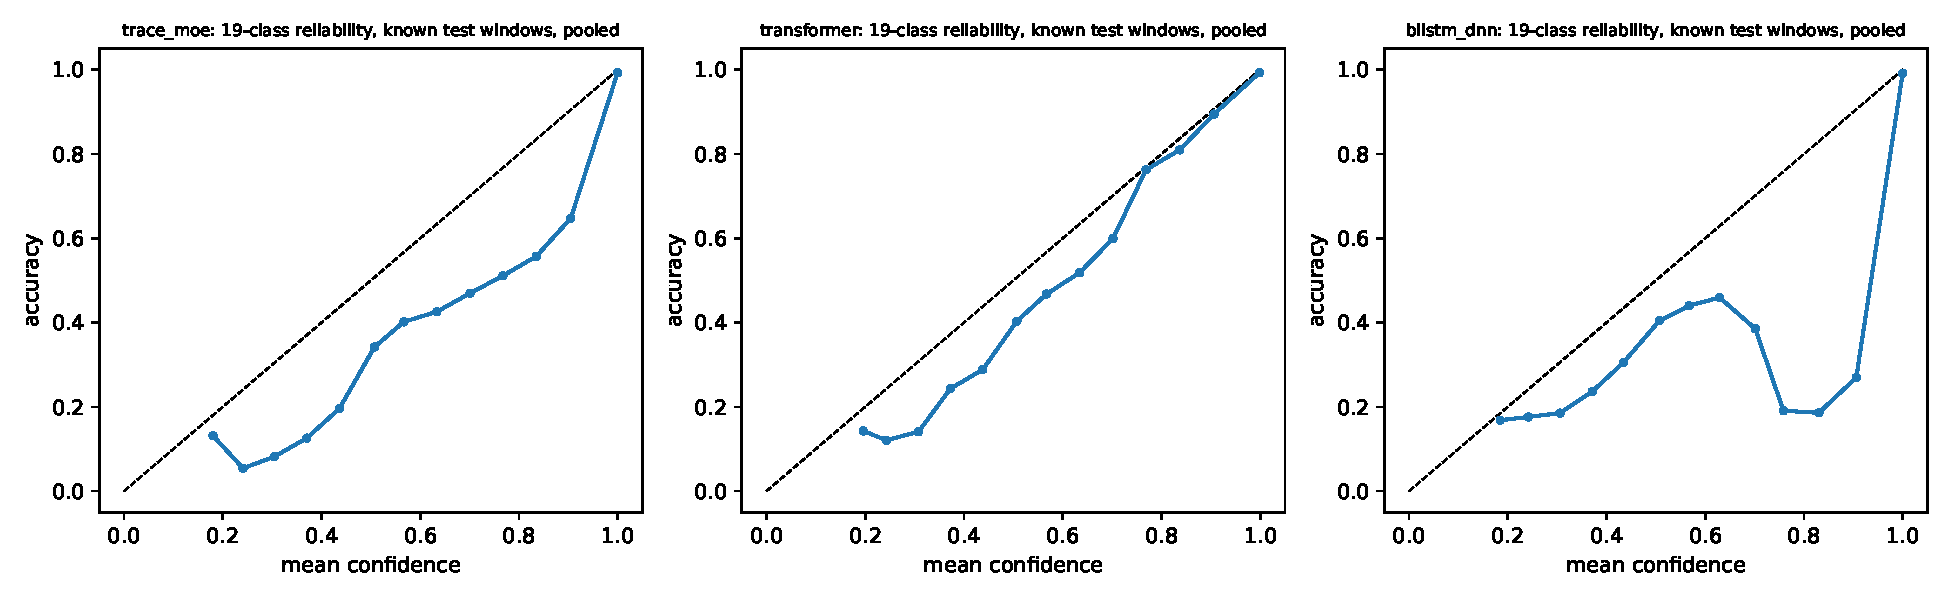
\includegraphics[width=0.92\linewidth]{figures/figS1-reliability.pdf}
\caption{Reliability diagram of the 19-class head on known test windows (15 equal-width confidence bins), per architecture, pooled over the held-out classes and seeds (exploratory; no verdict). The panel titles use the identifiers \texttt{trace\_moe}, \texttt{transformer} and \texttt{bilstm\_dnn} for TRACE-MoE, Transformer and BiLSTM-DNN.}\label{fig:figS1}
\end{figure}
\begin{figure}[!htbp]
\centering
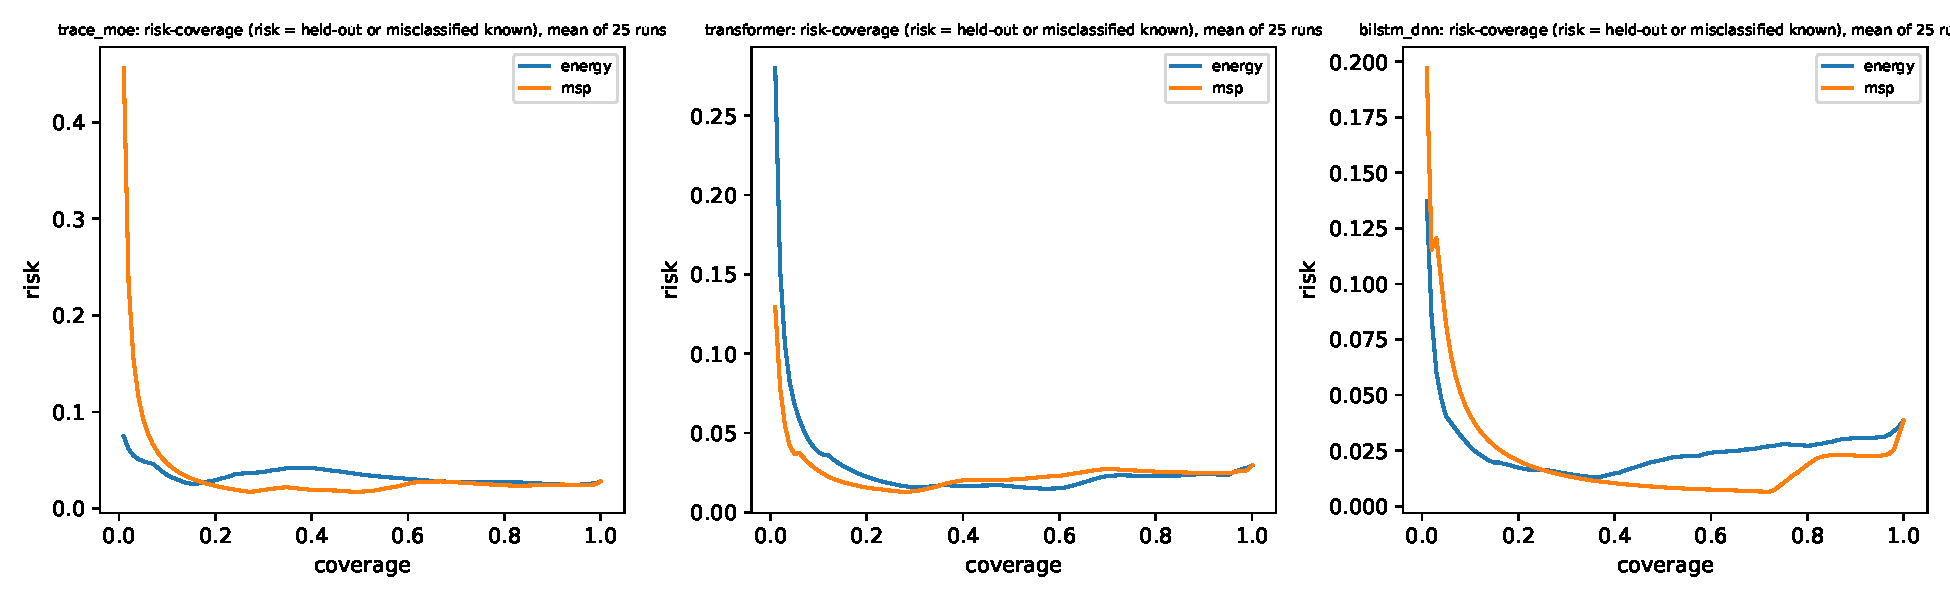
\includegraphics[width=0.92\linewidth]{figures/figS2-risk-coverage.pdf}
\caption{Risk-coverage curves when windows are accepted in order of increasing unknown score (energy score and MSP); held-out windows and misclassified known windows count as errors (exploratory; no verdict; the area under each curve is the AURC of Table~\ref{tab:S12}). Each curve is the mean of 25 runs; the panel titles use the identifiers \texttt{trace\_moe}, \texttt{transformer} and \texttt{bilstm\_dnn} for TRACE-MoE, Transformer and BiLSTM-DNN.}\label{fig:figS2}
\end{figure}

\section{Block bootstrap and flood sub-clusters}\label{sec:n11}
The seed-level intervals of the manuscript treat each test set as given. Table~\ref{tab:S13} (Panel A) adds a block bootstrap for the two flood classes; the held-out file of ARP spoofing, Recon-VulScan and malformed MQTT traffic is too short for a reliable block bootstrap, so no interval is reported for them. Panel B and Figure~\ref{fig:figS3} describe k-means sub-clusters of the held-out flood windows: the sub-clusters do not reveal a well-ranked subgroup that would explain the weakness of the energy score on these classes.
\begin{table}[!htbp]
\centering\scriptsize
\caption{Block bootstrap and flood sub-clusters (exploratory; no verdict). Panel A: block bootstrap for the two flood classes (2,000 resamples; seeds, the 20 known-class test files and blocks of 1,000, 250 or 4,000 consecutive held-out windows are resampled) next to the published 10,000-resample seed-level intervals; the held-out windows of each class come from a single test file, so dependence between capture files cannot be estimated. For ARP spoofing, Recon-VulScan and malformed MQTT traffic the held-out file is too short for a reliable block bootstrap and no interval is given. Panel B: k-means sub-clusters ($k = 2$ to 5, five seeds) of the held-out flood windows: mean silhouette, and the energy-score AUROC of each sub-cluster pooled over seeds and $k$ (min to max, window-weighted mean, share of sub-clusters below 0.5).}\label{tab:S13}
\textbf{Panel A}\par\smallskip
\fit{%
\begin{tabular}{llrcccc}
\toprule
Held-out class & Quantity & Mean & Published seed-level 95\% CI & Block, 1,000 & Block, 250 & Block, 4,000 \\
\midrule
TCP/IP DoS-UDP & H1 caught-any, TRACE-MoE & 1.0000 & [1.0000, 1.0000] & [1.0000, 1.0000] & [1.0000, 1.0000] & [1.0000, 1.0000] \\
TCP/IP DoS-UDP & H5 PCRP AUROC & 0.9513 & [0.9314, 0.9712] & [0.8860, 0.9978] & [0.8861, 0.9977] & [0.8864, 0.9978] \\
TCP/IP DoS-UDP & H2 energy minus MSP, TRACE-MoE & $-$0.1286 & [$-$0.2563, $-$0.0238] & [$-$0.3147, +0.0445] & [$-$0.3145, +0.0446] & [$-$0.3148, +0.0446] \\
TCP/IP DoS-UDP & H2 energy minus MSP, Transformer & +0.0888 & [+0.0010, +0.2091] & [$-$0.0094, +0.2540] & [$-$0.0095, +0.2539] & [$-$0.0093, +0.2543] \\
TCP/IP DoS-UDP & H2 energy minus MSP, BiLSTM-DNN & $-$0.0775 & [$-$0.2272, +0.0714] & [$-$0.3235, +0.1391] & [$-$0.3236, +0.1386] & [$-$0.3245, +0.1389] \\
\midrule
MQTT-DDoS publish flooding & H1 caught-any, TRACE-MoE & 1.0000 & [0.9999, 1.0000] & [0.9999, 1.0000] & [0.9999, 1.0000] & [0.9999, 1.0000] \\
MQTT-DDoS publish flooding & H5 PCRP AUROC & 0.9361 & [0.9360, 0.9363] & [0.8842, 0.9718] & [0.8838, 0.9716] & [0.8838, 0.9717] \\
MQTT-DDoS publish flooding & H2 energy minus MSP, TRACE-MoE & $-$0.0537 & [$-$0.1933, +0.0858] & [$-$0.2269, +0.1302] & [$-$0.2272, +0.1316] & [$-$0.2252, +0.1310] \\
MQTT-DDoS publish flooding & H2 energy minus MSP, Transformer & $-$0.1811 & [$-$0.2938, $-$0.0684] & [$-$0.3686, $-$0.0485] & [$-$0.3632, $-$0.0489] & [$-$0.3647, $-$0.0486] \\
MQTT-DDoS publish flooding & H2 energy minus MSP, BiLSTM-DNN & $-$0.1082 & [$-$0.2703, +0.0540] & [$-$0.2934, +0.0791] & [$-$0.2925, +0.0800] & [$-$0.2929, +0.0810] \\
\bottomrule
\end{tabular}
}
\par\medskip\textbf{Panel B}\par\smallskip
\fit{%
\begin{tabular}{llrrrrcrr}
\toprule
Held-out class & Model & Silhouette $k{=}2$ & $k{=}3$ & $k{=}4$ & $k{=}5$ & Energy AUROC per sub-cluster (min to max) & Window-weighted mean & Below 0.5 \\
\midrule
TCP/IP DoS-UDP & TRACE-MoE & 0.853 & 0.445 & 0.456 & 0.464 & 0.010 to 0.747 & 0.314 & 80\% \\
TCP/IP DoS-UDP & Transformer & 0.853 & 0.445 & 0.456 & 0.464 & 0.353 to 0.889 & 0.667 & 20\% \\
TCP/IP DoS-UDP & BiLSTM-DNN & 0.853 & 0.445 & 0.456 & 0.464 & 0.459 to 0.989 & 0.665 & 34\% \\
\midrule
MQTT-DDoS publish flooding & TRACE-MoE & 0.366 & 0.331 & 0.362 & 0.321 & 0.026 to 0.840 & 0.326 & 81\% \\
MQTT-DDoS publish flooding & Transformer & 0.366 & 0.331 & 0.362 & 0.321 & 0.003 to 0.771 & 0.116 & 89\% \\
MQTT-DDoS publish flooding & BiLSTM-DNN & 0.366 & 0.331 & 0.362 & 0.321 & 0.028 to 0.997 & 0.334 & 69\% \\
\bottomrule
\end{tabular}
}
\end{table}

\begin{figure}[!htbp]
\centering
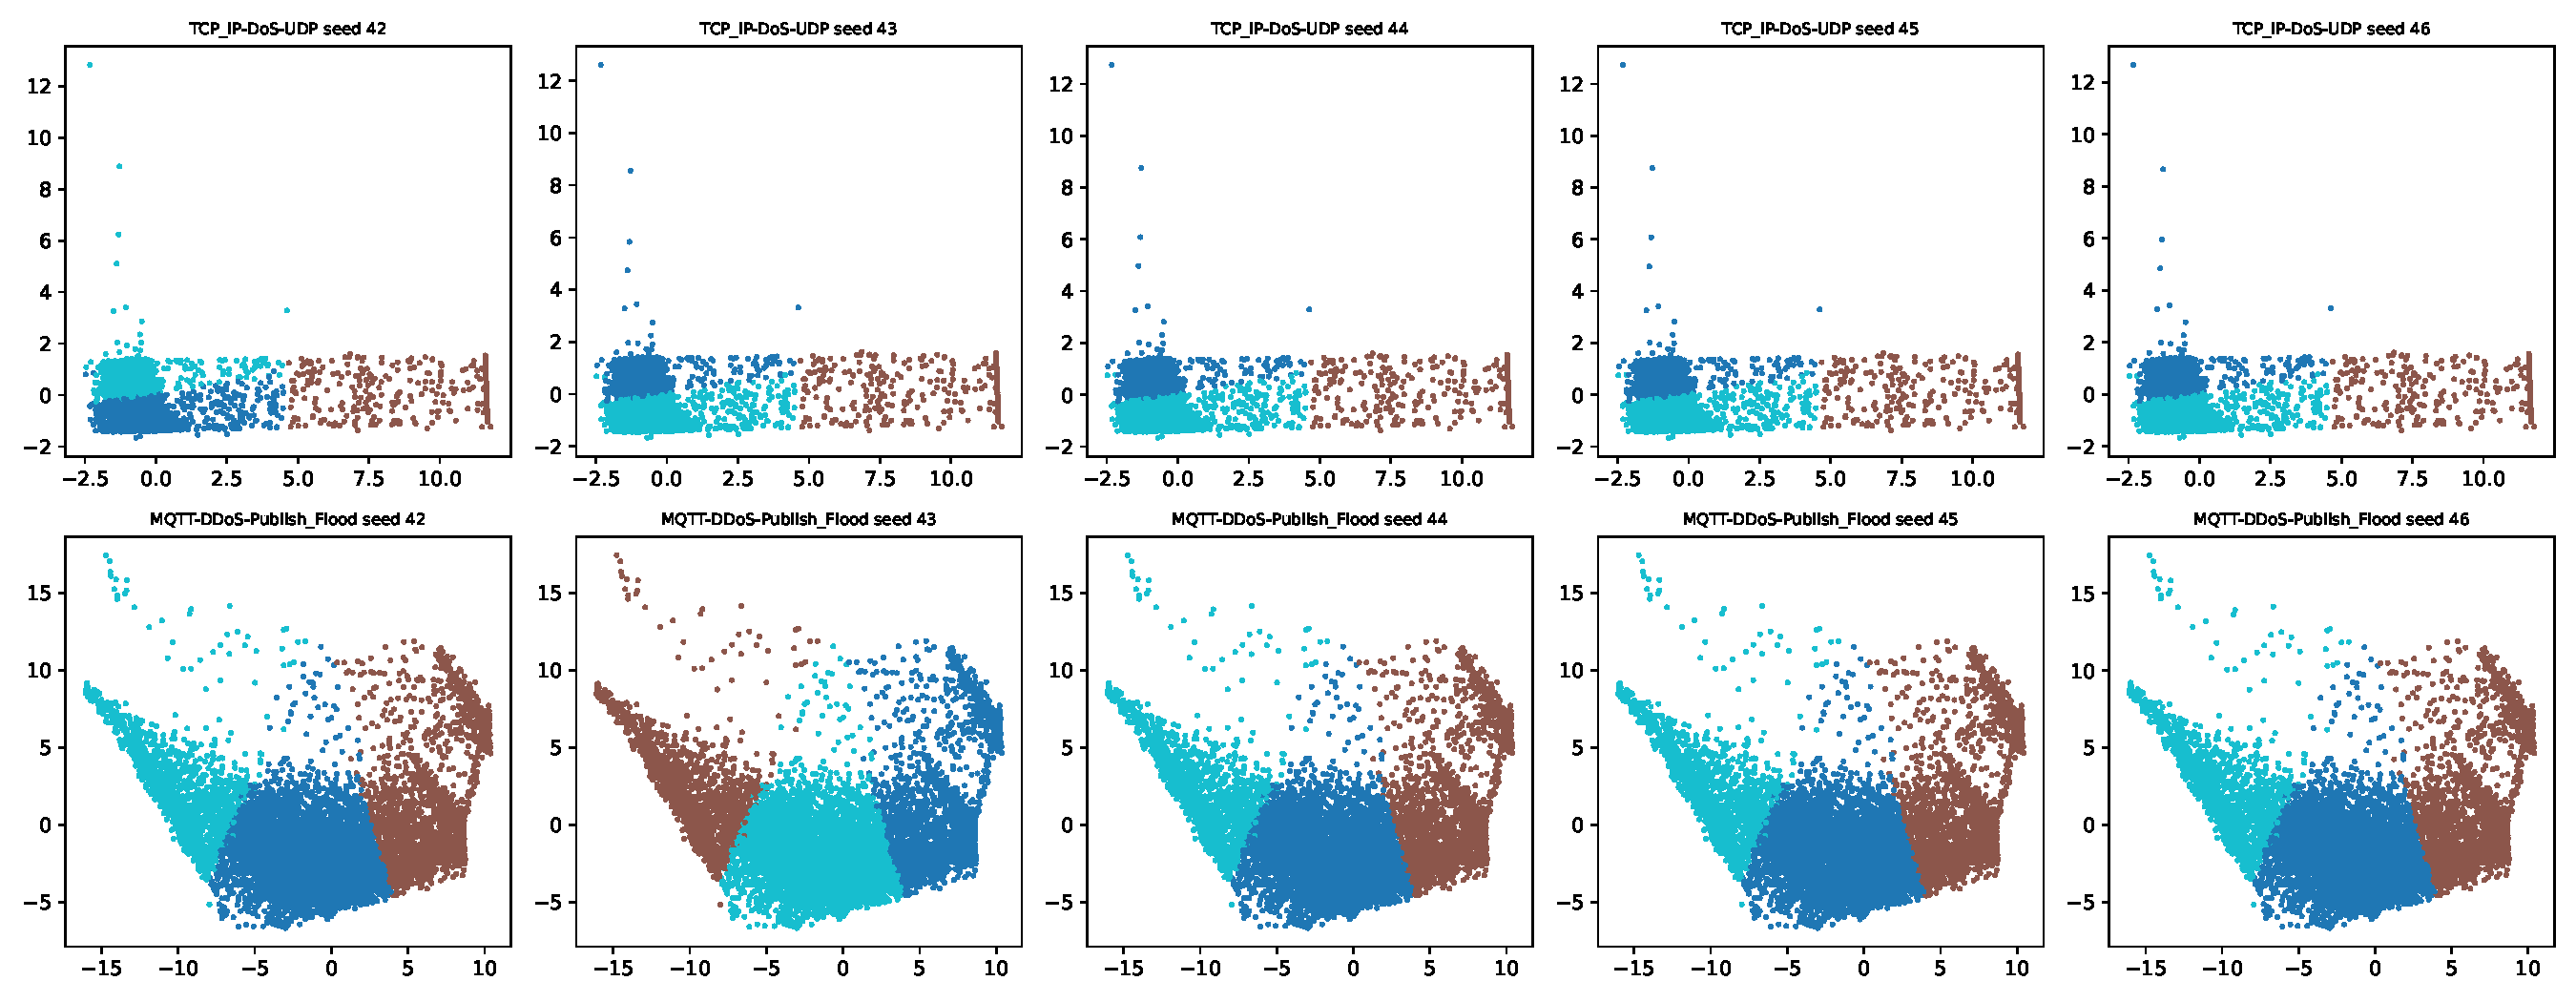
\includegraphics[width=0.92\linewidth]{figures/figS3-flood-subclusters.pdf}
\caption{Two-dimensional principal-component view of the k-means sub-clusters ($k = 3$) of the held-out flood windows, one panel per seed (exploratory; for inspection only; no verdict). Upper row: TCP/IP DoS-UDP; lower row: MQTT-DDoS publish flooding (panel titles use the identifiers \texttt{TCP\_IP-DoS-UDP} and \texttt{MQTT-DDoS-Publish\_Flood}).}\label{fig:figS3}
\end{figure}

\section{Coarser-head scores}\label{sec:n12}
Table~\ref{tab:S14} compares the MSP and the energy score of the 2-, 6- and 19-class heads as unknown-attack scores, computed from float32 head outputs of the saved models. The paired difference to the 19-class energy AUROC is given in parentheses, and an asterisk marks a 95\% seed interval that excludes zero. MSP cells in which most windows tie at the maximum value are marked with a dagger and are not interpreted. These analyses lie outside the pre-specified hypotheses.
\begin{table}[!htbp]
\centering\footnotesize
\caption{Energy and MSP of the 2-, 6- and 19-class heads as unknown-attack scores (exploratory; no verdict): AUROC for separating held-out windows from known-class test windows, per architecture and held-out class (mean over five seeds), from float32 head outputs of the saved models; the column labels give the score and the head (for example MSP 6 is the MSP of the 6-class head, Energy 19 the reference). The paired difference to the 19-class energy AUROC is given in parentheses.}\label{tab:S14}
\fit{%
\begin{tabular}{llrrrrrr}
\toprule
Model & Held-out class & Energy 19 & MSP 19 & MSP 6 & MSP 2 & Energy 6 & Energy 2 \\
\midrule
TRACE-MoE & ARP spoofing & 0.966 & 0.969$^{\dagger}$ (+0.003) & 0.933$^{\dagger}$ ($-$0.032) & 0.949$^{\dagger}$ ($-$0.017) & 0.969 (+0.004) & 0.971 (+0.005) \\
TRACE-MoE & Recon-VulScan & 0.969 & 0.971$^{\dagger}$ (+0.002) & 0.884$^{\dagger}$ ($-$0.085$^{*}$) & 0.816$^{\dagger}$ ($-$0.154$^{*}$) & 0.976 (+0.007$^{*}$) & 0.908 ($-$0.061$^{*}$) \\
TRACE-MoE & Malformed MQTT traffic & 0.981 & 0.982$^{\dagger}$ (+0.001) & 0.975$^{\dagger}$ ($-$0.006) & 0.975$^{\dagger}$ ($-$0.006) & 0.988 (+0.007$^{*}$) & 0.986 (+0.005) \\
TRACE-MoE & TCP/IP DoS-UDP & 0.314 & 0.442$^{\dagger}$ (+0.129$^{*}$) & 0.372$^{\dagger}$ (+0.058) & 0.454$^{\dagger}$ (+0.141) & 0.339 (+0.025$^{*}$) & 0.538 (+0.225$^{*}$) \\
TRACE-MoE & MQTT-DDoS publish flooding & 0.326 & 0.379$^{\dagger}$ (+0.054) & 0.387$^{\dagger}$ (+0.061) & 0.494$^{\dagger}$ (+0.168$^{*}$) & 0.398 (+0.072) & 0.308 ($-$0.018) \\
\midrule
Transformer & ARP spoofing & 0.982 & 0.961 ($-$0.021$^{*}$) & 0.978 ($-$0.004) & 0.989 (+0.007$^{*}$) & 0.987 (+0.005) & 0.989 (+0.007$^{*}$) \\
Transformer & Recon-VulScan & 0.974 & 0.934 ($-$0.040$^{*}$) & 0.877 ($-$0.098$^{*}$) & 0.859 ($-$0.115$^{*}$) & 0.976 (+0.002) & 0.848 ($-$0.126$^{*}$) \\
Transformer & Malformed MQTT traffic & 0.982 & 0.955 ($-$0.026$^{*}$) & 0.944 ($-$0.037$^{*}$) & 0.950 ($-$0.032$^{*}$) & 0.983 (+0.002$^{*}$) & 0.942 ($-$0.039$^{*}$) \\
Transformer & TCP/IP DoS-UDP & 0.667 & 0.579 ($-$0.089$^{*}$) & 0.673 (+0.006) & 0.254 ($-$0.413$^{*}$) & 0.592 ($-$0.076$^{*}$) & 0.299 ($-$0.368$^{*}$) \\
Transformer & MQTT-DDoS publish flooding & 0.116 & 0.297 (+0.181$^{*}$) & 0.158 (+0.042) & 0.238 (+0.123) & 0.507 (+0.391$^{*}$) & 0.208 (+0.092) \\
\midrule
BiLSTM-DNN & ARP spoofing & 0.857 & 0.975$^{\dagger}$ (+0.117$^{*}$) & 0.990$^{\dagger}$ (+0.133$^{*}$) & 0.995$^{\dagger}$ (+0.137$^{*}$) & 0.986 (+0.128$^{*}$) & 0.996 (+0.139$^{*}$) \\
BiLSTM-DNN & Recon-VulScan & 0.728 & 0.851$^{\dagger}$ (+0.124$^{*}$) & 0.797$^{\dagger}$ (+0.069$^{*}$) & 0.792$^{\dagger}$ (+0.064) & 0.821 (+0.093$^{*}$) & 0.956 (+0.228$^{*}$) \\
BiLSTM-DNN & Malformed MQTT traffic & 0.906 & 0.971$^{\dagger}$ (+0.065$^{*}$) & 0.967$^{\dagger}$ (+0.061$^{*}$) & 0.955$^{\dagger}$ (+0.050$^{*}$) & 0.960 (+0.055$^{*}$) & 0.990 (+0.085$^{*}$) \\
BiLSTM-DNN & TCP/IP DoS-UDP & 0.665 & 0.743$^{\dagger}$ (+0.078) & 0.691$^{\dagger}$ (+0.026) & 0.484$^{\dagger}$ ($-$0.181$^{*}$) & 0.758 (+0.093$^{*}$) & 0.753 (+0.088) \\
BiLSTM-DNN & MQTT-DDoS publish flooding & 0.334 & 0.442$^{\dagger}$ (+0.108) & 0.541$^{\dagger}$ (+0.207$^{*}$) & 0.520$^{\dagger}$ (+0.186$^{*}$) & 0.640 (+0.306$^{*}$) & 0.520 (+0.186$^{*}$) \\
\bottomrule
\end{tabular}
}
\par\smallskip{\footnotesize $^{\dagger}$ MSP tie share of 0.5 or more among the held-out or the known windows (share of windows whose MSP is exactly 1.0 in float32): 30 of 45 MSP cells; in these cells the larger of the two tie shares is 0.52 to 1.00. The Transformer has no marked cell (largest tie share 0.18). $^{*}$ The 95\% seed interval of the paired difference to the 19-class energy AUROC excludes zero. All cells are shown, including those that are not interpretable.}
\end{table}


\section{Benign-calibrated thresholds}\label{sec:n13}
Table~\ref{tab:S15} shows the effect of setting the abstention threshold at a low percentile of the validation energy of Benign windows only (1,806 Benign validation windows per run, so the 1\% threshold rests on about 18 windows) instead of the 5th percentile of all validation windows (reference). A window is flagged when its energy is below the threshold, and the safety-view alert adds the binary head. Panel B gives TRACE-MoE per class and Panel C the event rules. No threshold is recommended.
\begin{table}[!htbp]
\centering\footnotesize
\caption{Benign-calibrated abstention thresholds (exploratory; descriptive; no verdict; no threshold is recommended). The reference threshold is the 5th percentile of all validation energies; the other thresholds are the 1st, 2nd and 5th percentile of the validation energy of Benign windows only; all thresholds use validation windows only. A window is flagged when its energy is below the threshold, and the safety-view alert adds the binary head (attack probability above 0.5). Panel A: Benign alert rate (safety view), held-out caught-any rate and false-alarm rate of the energy flag on all known test windows, mean over the five classes with a 95\% bootstrap interval over the five seed means. Panel B: caught-any rate of TRACE-MoE per held-out class (mean over five seeds with 95\% interval). Panel C: event rules (at least $m$ of the last $n$ windows of a capture file): Benign events per 10,000 Benign windows and share of held-out windows that trigger among those with a full history, means over classes and seeds; events count alarm onsets, so a lower alert rate can give more separate events.}\label{tab:S15}
\textbf{Panel A: all classes}\par\smallskip
\fit{%
\begin{tabular}{llccc}
\toprule
Model & Threshold & Benign alert rate (safety view) & Held-out caught-any & Known false-alarm rate (energy flag) \\
\midrule
TRACE-MoE & Reference & 0.8833 [0.8202, 0.9464] & 0.9836 [0.9555, 0.9987] & 0.0418 [0.0399, 0.0447] \\
TRACE-MoE & Benign 1st pct & 0.0428 [0.0331, 0.0528] & 0.7232 [0.7066, 0.7457] & 0.0027 [0.0020, 0.0034] \\
TRACE-MoE & Benign 2nd pct & 0.0560 [0.0466, 0.0653] & 0.7549 [0.7390, 0.7777] & 0.0052 [0.0028, 0.0089] \\
TRACE-MoE & Benign 5th pct & 0.0890 [0.0806, 0.0963] & 0.8064 [0.7851, 0.8276] & 0.0126 [0.0050, 0.0262] \\
\midrule
Transformer & Reference & 0.9973 [0.9966, 0.9980] & 0.9988 [0.9977, 0.9995] & 0.0440 [0.0427, 0.0455] \\
Transformer & Benign 1st pct & 0.0560 [0.0455, 0.0644] & 0.7129 [0.6899, 0.7353] & 0.0013 [0.0007, 0.0024] \\
Transformer & Benign 2nd pct & 0.0673 [0.0560, 0.0762] & 0.7453 [0.7229, 0.7677] & 0.0021 [0.0010, 0.0037] \\
Transformer & Benign 5th pct & 0.0994 [0.0871, 0.1098] & 0.8049 [0.7832, 0.8239] & 0.0033 [0.0021, 0.0053] \\
\midrule
BiLSTM-DNN & Reference & 0.5015 [0.4319, 0.5795] & 0.9172 [0.8704, 0.9585] & 0.0510 [0.0448, 0.0554] \\
BiLSTM-DNN & Benign 1st pct & 0.0784 [0.0758, 0.0814] & 0.6902 [0.6694, 0.7096] & 0.0056 [0.0013, 0.0136] \\
BiLSTM-DNN & Benign 2nd pct & 0.0912 [0.0874, 0.0949] & 0.7024 [0.6822, 0.7233] & 0.0064 [0.0021, 0.0145] \\
BiLSTM-DNN & Benign 5th pct & 0.1293 [0.1233, 0.1352] & 0.7453 [0.7199, 0.7684] & 0.0087 [0.0043, 0.0166] \\
\bottomrule
\end{tabular}
}
\par\medskip\textbf{Panel B: TRACE-MoE per held-out class, held-out caught-any}\par\smallskip
\fit{%
\begin{tabular}{lcccc}
\toprule
TRACE-MoE, held-out class & Reference & Benign 1st pct & Benign 2nd pct & Benign 5th pct \\
\midrule
ARP spoofing & 0.9239 [0.7808, 0.9992] & 0.5158 [0.4326, 0.6330] & 0.5717 [0.4644, 0.6984] & 0.6554 [0.5240, 0.7910] \\
Recon-VulScan & 0.9998 [0.9994, 1.0000] & 0.6600 [0.6268, 0.6933] & 0.6998 [0.6673, 0.7297] & 0.7746 [0.7431, 0.8022] \\
Malformed MQTT traffic & 0.9941 [0.9858, 1.0000] & 0.4404 [0.3901, 0.4860] & 0.5033 [0.4553, 0.5543] & 0.6018 [0.5580, 0.6548] \\
TCP/IP DoS-UDP & 1.0000 [1.0000, 1.0000] & 1.0000 [1.0000, 1.0000] & 1.0000 [1.0000, 1.0000] & 1.0000 [1.0000, 1.0000] \\
MQTT-DDoS publish flooding & 1.0000 [0.9999, 1.0000] & 0.9999 [0.9998, 1.0000] & 0.9999 [0.9998, 1.0000] & 0.9999 [0.9998, 1.0000] \\
\bottomrule
\end{tabular}
}
\par\medskip\textbf{Panel C: event rules}\par\smallskip
\fit{%
\begin{tabular}{llrrrrrr}
\toprule
Model & Threshold & 2 of 4: events & triggering & 8 of 16: events & triggering & 32 of 64: events & triggering \\
\midrule
TRACE-MoE & Reference & 25.94 & 0.9965 & 8.58 & 0.9964 & 2.30 & 0.9978 \\
TRACE-MoE & Benign 1st pct & 61.19 & 0.7935 & 14.71 & 0.7576 & 2.70 & 0.7477 \\
TRACE-MoE & Benign 2nd pct & 79.54 & 0.8271 & 20.15 & 0.7953 & 4.37 & 0.8032 \\
TRACE-MoE & Benign 5th pct & 113.91 & 0.8803 & 33.19 & 0.8611 & 7.93 & 0.8797 \\
\midrule
Transformer & Reference & 1.09 & 0.9999 & 0.28 & 1.0000 & 0.27 & 1.0000 \\
Transformer & Benign 1st pct & 58.39 & 0.7765 & 15.56 & 0.7241 & 3.21 & 0.7072 \\
Transformer & Benign 2nd pct & 77.37 & 0.8113 & 20.71 & 0.7683 & 3.92 & 0.7634 \\
Transformer & Benign 5th pct & 106.13 & 0.8797 & 35.09 & 0.8547 & 9.26 & 0.8733 \\
\midrule
BiLSTM-DNN & Reference & 212.45 & 0.9629 & 64.07 & 0.9526 & 18.67 & 0.9484 \\
BiLSTM-DNN & Benign 1st pct & 145.96 & 0.7465 & 31.97 & 0.6876 & 8.08 & 0.6581 \\
BiLSTM-DNN & Benign 2nd pct & 158.26 & 0.7631 & 31.86 & 0.7053 & 7.29 & 0.6819 \\
BiLSTM-DNN & Benign 5th pct & 207.16 & 0.8155 & 41.75 & 0.7696 & 9.85 & 0.7736 \\
\bottomrule
\end{tabular}
}
\end{table}


\FloatBarrier
\section{Result figures}\label{sec:n14}
Figures~\ref{fig:figS4} to~\ref{fig:figS7} reproduce the result figures of the hypotheses H1, H2, H4 and H5; each caption names the manuscript table whose values it shows.
\begin{figure}[!htbp]
\centering
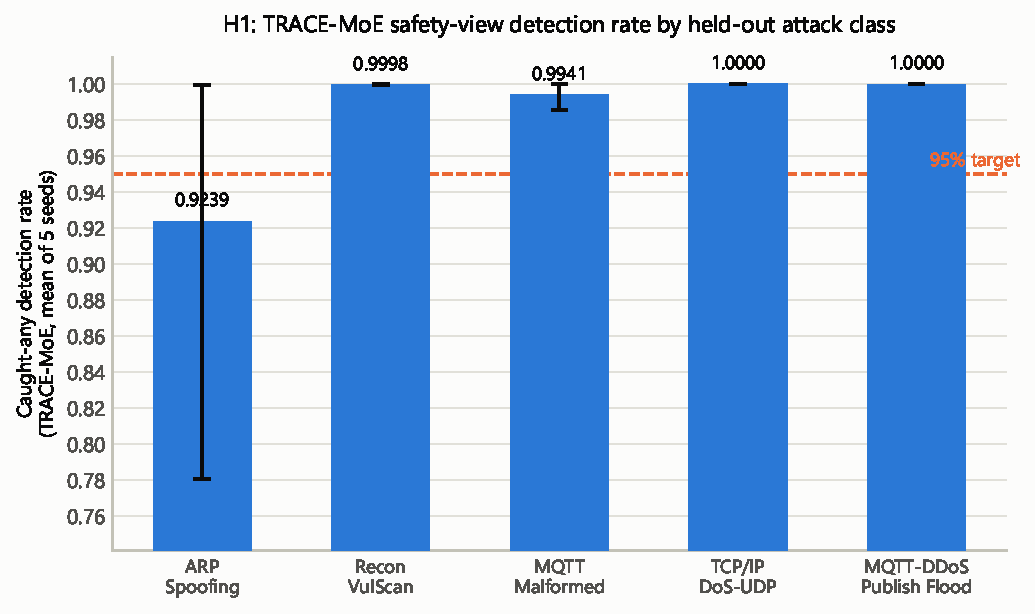
\includegraphics[width=0.92\linewidth]{figures/figS4-h1-safety-view.pdf}
\caption{Safety-view (caught-any) detection rate of TRACE-MoE per held-out class: bars show the mean over five seeds and error bars the bootstrap 95\% confidence interval; the dashed line is the 0.95 target; the values are those of Table 1 of the manuscript (descriptive; the verdicts are those of the manuscript).}\label{fig:figS4}
\end{figure}
\begin{figure}[!htbp]
\centering
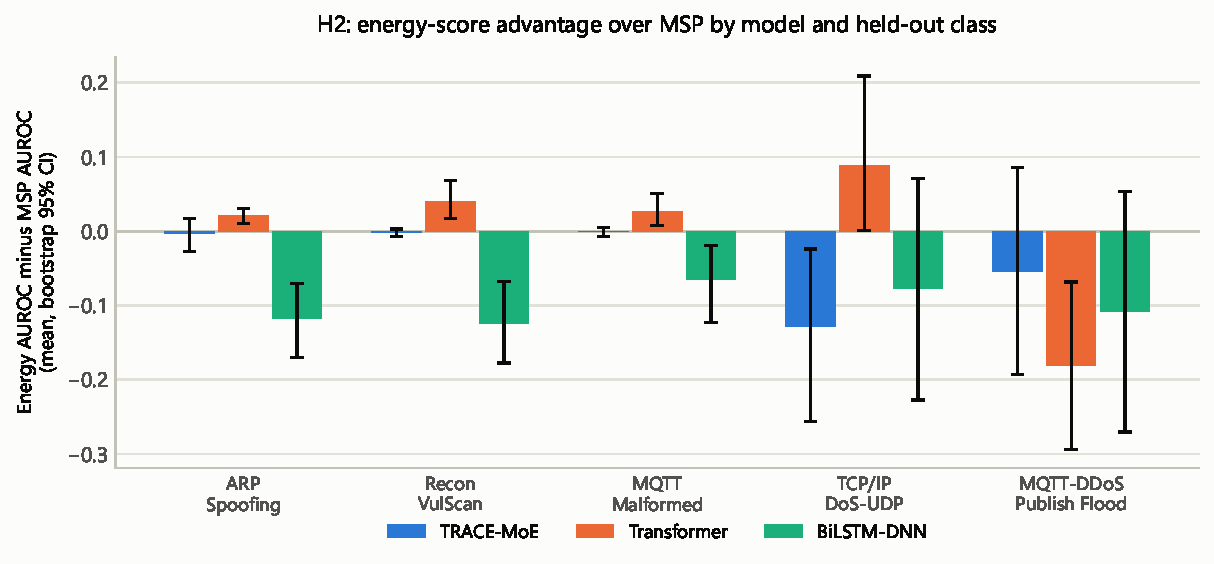
\includegraphics[width=0.92\linewidth]{figures/figS5-h2-energy-vs-msp.pdf}
\caption{Energy-score minus MSP AUROC per architecture and held-out class: bars show the mean over five seeds and error bars the bootstrap 95\% confidence interval; the values are those of Table 3 of the manuscript (descriptive; the verdicts are those of the manuscript).}\label{fig:figS5}
\end{figure}
\begin{figure}[!htbp]
\centering
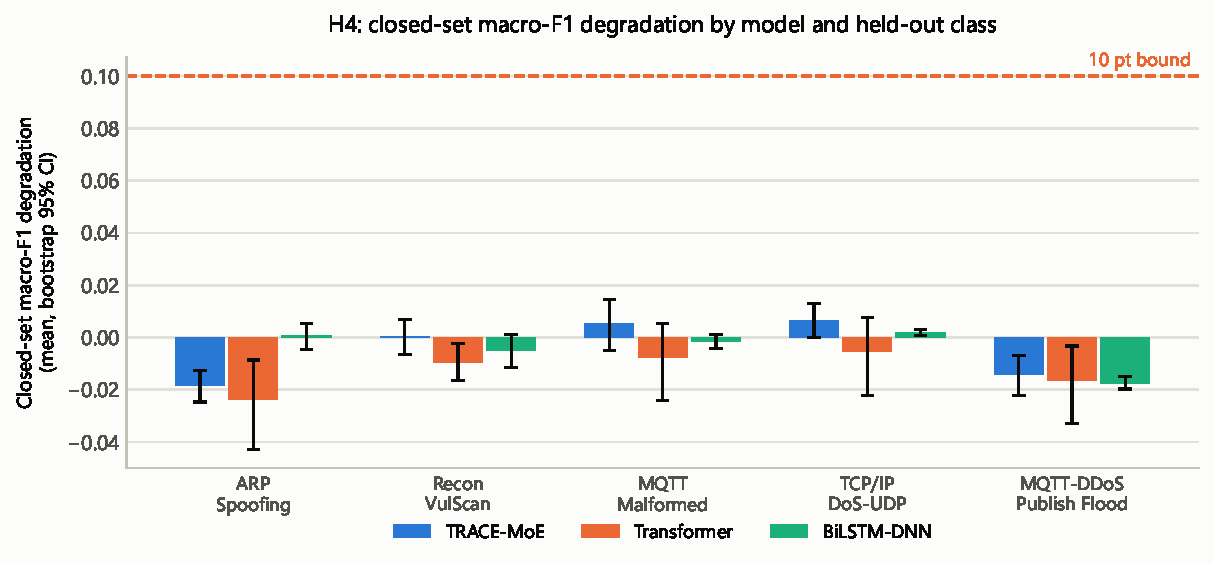
\includegraphics[width=0.92\linewidth]{figures/figS6-h4-closed-set-degradation.pdf}
\caption{Closed-set macro-F1 degradation per architecture and held-out class against the 10-percentage-point bound (dashed line): bars show the mean over five seeds and error bars the bootstrap 95\% confidence interval; the values are those of Table 4 of the manuscript (descriptive; the verdicts are those of the manuscript).}\label{fig:figS6}
\end{figure}
\begin{figure}[!htbp]
\centering
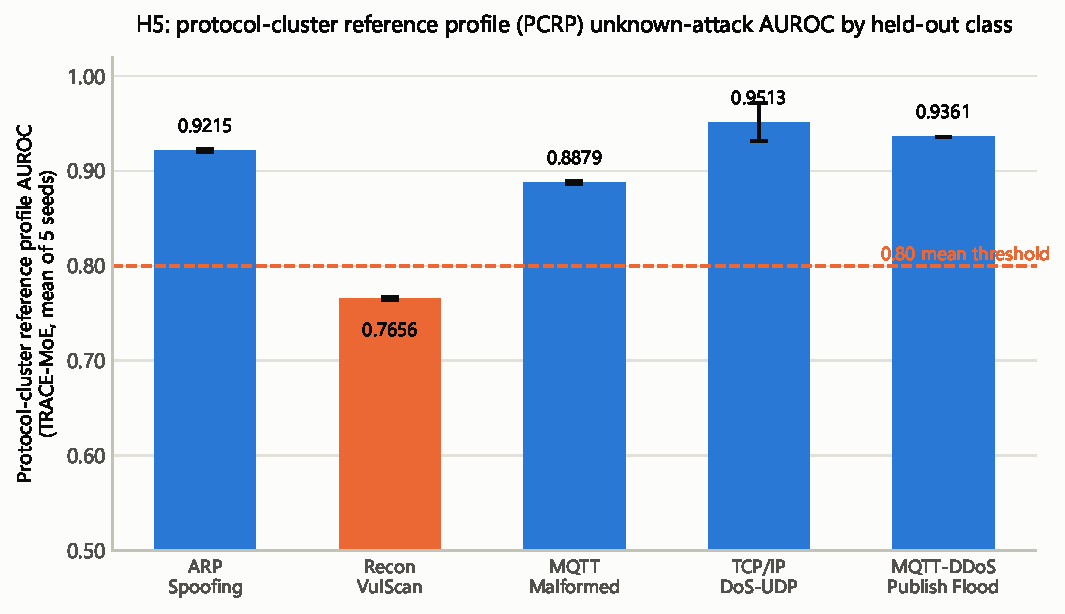
\includegraphics[width=0.92\linewidth]{figures/figS7-h5-pcrp-auroc.pdf}
\caption{Unknown-attack ranking AUROC of the protocol-cluster reference profile (PCRP) per held-out class: bars show the mean over five seeds and error bars the bootstrap 95\% confidence interval; the dashed line is the 0.80 mean threshold; the values are those of Table 5 of the manuscript (descriptive; the verdicts are those of the manuscript).}\label{fig:figS7}
\end{figure}

\section{Reproducibility}\label{sec:n15}
The table below lists the software used for table generation and the training and benchmark environment. All 75 models were trained with seeds 42 to 46 on one workstation (see the manuscript section on hardware). The scripts used for the analyses are listed with the first 16 characters of their SHA-256 hash.

\begin{center}\small
\begin{tabular}{p{6.2cm}p{7cm}}
\toprule
Item & Value \\
\midrule
Python & 3.12.4 \\
numpy / pandas (table generation) & 2.5.3 / 3.0.6 \\
PyTorch / CUDA (training and benchmark) & 2.5.1+cu121 / 12.1 \\
GPU & NVIDIA GeForce RTX 3050 Laptop GPU \\
Platform & Windows-11-10.0.26300-SP0 \\
\bottomrule
\end{tabular}
\end{center}

\begin{center}\footnotesize
\begin{tabular}{p{4.9cm}p{6.6cm}l}
\toprule
Purpose & Script & SHA-256 (first 16) \\
\midrule
Training and evaluation of the 75 leave-one-attack-out runs & 07\_unknown\_attacks.py & 3978c2ed442f3a6c \\
Export of per-window scores from the saved models & p4\_export\_scores.py & 485cf46a2b4fde30 \\
Safety-view decomposition (Tables~\ref{tab:S4}, \ref{tab:S5}) & p4\_analyze\_exports.py & 13748d3bbb402afc \\
Inference benchmark (Table~\ref{tab:S3}) & p4\_inference\_benchmark.py & e235bf0bfa659aa6 \\
Hypothesis verdicts and ESA1 (Table~\ref{tab:S6}) & paper4\_h8\_verdict.py & 9812c64ec77e40bd \\
PCRP profiles and scores & 24\_twin\_score\_paper4.py & 7a5108a7a68626a8 \\
PCRP verdicts & 25\_twin\_verdict\_paper4.py & 77651a1354b133d2 \\
Benign flag rates (Table~\ref{tab:S7} (Panel A)) & p4\_rev\_v4\_benign\_disclosure.py & acd9ef57a4749357 \\
Safety-view alerts and AURC (Tables~\ref{tab:S7} (Panel A), \ref{tab:S12}) & p4\_rev\_t5\_t9.py & 2bcdea256397197b \\
Event-level rule (Table~\ref{tab:S7} (Panel B)) & p4\_rev\_9\_event\_level.py & 35836aace6536116 \\
Spearman agreement (Table~\ref{tab:S8}) & p4\_rev\_saved\_scores.py & 5189b8f69c915188 \\
Feature-space scores (Table~\ref{tab:S9}) & p4\_rev\_t3\_feature\_scores.py & 5ccad28aed645375 \\
Feature-space score summary (Table~\ref{tab:S9}) & p4\_rev\_t3\_summarize.py & 735d3ca7900ab854 \\
Logit scores (Table~\ref{tab:S9}) & p4\_rev2\_10\_logit\_scores.py & c072a36463fac13c \\
Head-disagreement scores (Table~\ref{tab:S9}) & p4\_rev2\_2\_head\_disagreement.py & 53850dd9977cdd4d \\
Pooled score table (Table~\ref{tab:S9}) & p4\_rev2\_pooled\_table.py & fcf80c3c02e7d203 \\
PCRP estimators and aggregation (Table~\ref{tab:S11}) & p4\_rev\_pcrp\_t4\_u3.py & 1328fbd64f1091c3 \\
PCRP variant summary (Table~\ref{tab:S11}) & p4\_rev\_t4\_summarize.py & 6a3d98bf32e7e63a \\
Block bootstrap (Table~\ref{tab:S13}) & p4\_rev\_t6b\_block\_bootstrap.py & 00b91301f26b6ef6 \\
Flood sub-clusters (Table~\ref{tab:S13}) & p4\_rev\_t10\_flood\_clusters.py & 31e7072943d58df9 \\
Operating points and temperature (Table~\ref{tab:S10}) & p4\_rev\_2\_operating\_points.py & e2f5cdc946c96811 \\
Calibration (Table~\ref{tab:S12}) & p4\_rev\_5\_calibration\_risk\_coverage.py & 5fa676ff02a26022 \\
Float32 export of the head outputs (Table~\ref{tab:S14}) & p4\_rev2\_13b\_coarse\_head\_export.py & a5029b4edc4d642b \\
Coarser-head scores (Table~\ref{tab:S14}) & p4\_rev2\_13c\_coarse\_head\_scores.py & 85016b3bfcfe8da7 \\
Benign-calibrated thresholds (Table~\ref{tab:S15}) & p4\_rev\_r4\_benign\_threshold.py & 7ffb47138b589cb1 \\
\bottomrule
\end{tabular}
\end{center}

\end{document}
